%!TEX program = xelatex
\documentclass{beamer}
\usepackage[UTF8]{ctex}
\usepackage{lmodern}
\usepackage{bm}
\mode<presentation> {
	
	% The Beamer class comes with a number of default slide themes
	% which change the colors and layouts of slides. Below this is a list
	% of all the themes, uncomment each in turn to see what they look like.
	
	%\usetheme{default}
	%\usetheme{AnnArbor}
	%\usetheme{Antibes}
	%\usetheme{Bergen}
	%\usetheme{Berkeley}
	%\usetheme{Berlin}
	%\usetheme{Boadilla}
	%\usetheme{CambridgeUS}
	\usetheme{Copenhagen}
	%\usetheme{Darmstadt}
	%\usetheme{Dresden}
	%\usetheme{Frankfurt}
	%\usetheme{Goettingen}
	%\usetheme{Hannover}
	%\usetheme{Ilmenau}
	%\usetheme{JuanLesPins}
	%\usetheme{Luebeck}
	%\usetheme{Madrid}
	%\usetheme{Malmoe}
	%\usetheme{Marburg}
	%\usetheme{Montpellier}
	%\usetheme{PaloAlto}
	%\usetheme{Pittsburgh}
	%\usetheme{Rochester}
	%\usetheme{Singapore}
	%\usetheme{Szeged}
	%\usetheme{Warsaw}
	
	% As well as themes, the Beamer class has a number of color themes
	% for any slide theme. Uncomment each of these in turn to see how it
	% changes the colors of your current slide theme.
	
	%\usecolortheme{albatross}
	%\usecolortheme{beaver}
	%\usecolortheme{beetle}
	%\usecolortheme{crane}
	%\usecolortheme{dolphin}
	%\usecolortheme{dove}
	%\usecolortheme{fly}
	%\usecolortheme{lily}
	%\usecolortheme{orchid}
	%\usecolortheme{rose}
	%\usecolortheme{seagull}
	%\usecolortheme{seahorse}
	%\usecolortheme{whale}
	%\usecolortheme{wolverine}
	
	%\setbeamertemplate{footline} % To remove the footer line in all slides uncomment this line
	%\setbeamertemplate{footline}[page number] % To replace the footer line in all slides with a simple slide count uncomment this line
	
	%\setbeamertemplate{navigation symbols}{} % To remove the navigation symbols from the bottom of all slides uncomment this line
}

\usepackage{graphicx} % Allows including images
\usepackage{booktabs} % Allows the use of \toprule, \midrule and \bottomrule in tables 
\usepackage[T1]{fontenc}
\usepackage{tabularray}
\UseTblrLibrary{booktabs}
\usepackage[utf8]{inputenc}
\setbeamertemplate{caption}[numbered]
\newcommand{\C}{\mathbb{C}}
\newcommand{\R}{\mathbb{R}}
\newcommand{\Q}{\mathbb{Q}}
\newcommand{\Z}{\mathbb{Z}}
\newcommand{\N}{\mathbb{N}}
\newcommand{\p}{\mathbb{P}}
\newcommand{\E}{\mathbb{E}}
\newcommand{\new}[1]{\textcolor{red}{#1}}
\usepackage{graphicx}
\usepackage{amssymb}
\usepackage{setspace}
\usepackage[toc,page]{appendix}
\usepackage{epstopdf}
\usepackage{latexsym}
\usepackage{amstext}
\usepackage{lmodern}
\usepackage{amsmath}
\usepackage{bbm}
\usepackage{amsfonts}
\usepackage{url}
\usepackage{bm}
\usepackage{mathrsfs}
\usepackage{mathtools}
\usepackage{float}
%\usepackage{hyperref} give reference hyperlink 
%\usepackage{setspace}
\usepackage{indentfirst}
\usepackage{multirow}
\usepackage{color}
\usepackage{mathtools}
% packages from template
\usepackage{amsmath,amsthm,amssymb,amsfonts}
\usepackage[width=.9\textwidth]{caption}
\usepackage{mathrsfs}
\usepackage{graphicx}
\newcommand{\indep}{\rotatebox[origin=c]{90}{$\models$}}
%\usepackage{textgreek}
\usepackage{bbold}
\usepackage{subcaption}
\usepackage{natbib}
\usepackage{verbatim}
\usepackage{soul}
\usepackage[utf8]{inputenc}
%\usepackage[algo2e,ruled,vlined]{algorithm2e} 
%\usepackage{fancyvrb}


\newtheorem{proposition}[theorem]{Proposition}

\newcommand{\M}{\boldsymbol{M}}
\newcommand{\rank}{\mathrm{rank}}
\newcommand{\rep}{\mathrm{rep}}
\newcommand{\PR}{\text{Pr}}
\newcommand{\pkg}[1]{{\fontseries{b}\selectfont #1}}
%\newcommand\norm[1]{\left\lVert#1\right\rVert}
\newcommand{\bs}[1]{\pmb{#1}}
\newcommand{\mb}[1]{\boldsymbol{#1}}
\DeclareMathOperator*{\argmin}{arg\,min}
\DeclarePairedDelimiter{\ceil}{\lceil}{\rceil}
\DeclarePairedDelimiterX{\norm}[1]{\lVert}{\rVert}{#1}
\allowdisplaybreaks
%=============================================================================
% prelude
%=============================================================================
\def\mathLarge#1{\mbox{\LARGE $#1$}}
\usepackage{soul}


\title[]{随机变量及其概率分布}
\author[概率统计]{张宏达}
\institute{Nanjing University}
\date{}
\begin{document}
	\begin{frame}
		\titlepage
	\end{frame}
	
	\begin{frame}
		\frametitle{主要内容}
		\begin{itemize}
			\item 随机变量及其分布函数
			\item 离散随机变量及其分布
			\item 连续随机变量及其分布
			\item 随机变量函数的分布
		\end{itemize}
	\end{frame}
	
	\begin{frame}
		\frametitle{随机变量及其分布函数}
		定义 2.1 设 $\Omega=\{e\}$ 是随机试验的样本空间, 如果对每个 $e \in \Omega$, 都对应一个单值实函 数 $X=X(e)$, 称 $X$ 为随机变量。
		
		\vspace*{1cm}
%		我们一般以大写字母 $X, Y, Z$ 等表示随机变量, 以相对应的小写字母 $x, y, z$ 等表示随机变量的取值。例如用$X = x$代表在一次随机试验中观测到随机变量$X$取值为$x$。
		
		\vspace*{1cm}
		例 2.1 抛一枚骰子, 抛出的点数记为 $X$, 则 $X$ 是一个随机变量。 $X$ 的可能取值范 围是 $1,2,3,4,5,6$ 。 $\{X=1\}$ 表示随机事件 “抛出 1 点”, $\{X \geqslant 5\}$ 表示随机事件 “抛出 5 或 6 点”, $\{X=\pi\}$ 也是一个随机事件: 不可能事件。
		
		\vspace*{1cm}
		\textbf{概率分布}被用以描述随机变量取值的概率规律。
	\end{frame}
	
	\begin{frame}
		定义 2.2 设 $X$ 是一个随机变量, $x$ 是任意实数, 称函数
		
		$$
		F(x)=P(X \leqslant x), \quad-\infty<x<\infty
		$$
		
		为随机变量 $X$ 的\textbf{分布函数}。
		
		\vspace*{1cm}
		例 2.2 某人射击命中率为 0.6 , 独立射击 2 枪, 命中 $X$ 枪, 求 $X$ 的分布函数。
	\end{frame}
	
	\begin{frame}
		解:因为每次射击有命中和不命中两种结果,并且为独立重复试验,则其符合$n$重伯努利试验。根据定理 1.5可知
		\begin{align}
			& P(X=0)=(1-0.6)^{2}=0.16, \\
			& P(X=1)=C_{2}^{1} \cdot 0.6 \cdot(1-0.6)=0.48, \\
			& P(X=2)=0.6^{2}=0.36
		\end{align}
		
		根据分布函数定义及概率可加性有
		
		当 $x<0$ 时, $X \leqslant x$ 是不可能事件, $F(x)=P(X \leqslant x)=0$;
		
		当 $0 \leqslant x<1$ 时, $X \leqslant x \Leftrightarrow X=0, F(x)=P(X \leqslant x)=P(X=0)=0.16$;
		
		当 $1 \leqslant x<2$ 时, $X \leqslant x \Leftrightarrow\{X=0\} \cup\{X=1\}$,
		
		$$
		F(x)=P(X \leqslant x)=P(X=0)+P(X=1)=0.16+0.48=0.64 ;
		$$
		
		当 $x \geqslant 2$ 时, $X \leqslant x$ 是必然事件, $F(x)=P(X \leqslant x)=1$ 。
		
	\end{frame}
	
	\begin{frame}
		因此有
		$$
		F(x)=\left\{\begin{array}{cc}
			0, & x<0 \\
			0.16, & 0 \leqslant x<1 \\
			0.64, & 1 \leqslant x<2 \\
			1, & x \geqslant 2
		\end{array} .\right.
		$$
	\end{frame}
	
	\begin{frame}
		有了随机变量 $X$ 的分布函数 $F(x)$, 就可以用其描述 $X$ 在某些范围取值的概率, 如对 任意实数 $a, b(a<b)$ 有
		
		$$
		\begin{aligned}
			& P(a<X \leqslant b)=P(X \leqslant b)-P(X \leqslant a)=F(b)-F(a), \\
			& P(X>b)=1-P(X \leqslant b)=1-F(b) \\
			& P(X \geqslant b)=1-P(X<b)=1-F(b-0)
		\end{aligned}
		$$
	\end{frame}
		
	\begin{frame}
		分布函数 $F(x)$ 有如下\textbf{基本性质}:
		
		(1) $F(x)$ 为单调不减函数, 即对任意实数 $x_{2}>x_{1}$, 有 $F\left(x_{2}\right) \geqslant F\left(x_{1}\right)$ 。
		
		
		(2) $0 \leqslant F(x) \leqslant 1$, 且 $F(-\infty)=\lim _{x \rightarrow-\infty} F(x)=0, F(+\infty)=\lim _{x \rightarrow+\infty} F(x)=1$ 。
		
		(3) $F(x)$ 为右连续, 即 $F\left(x_{0}+0\right)=\lim _{x \rightarrow x_{0}+0} F(x)=F\left(x_{0}\right)$ 。
		
		任一随机变量的分布函数 $F(x)$ 必满足以上三性质。反之, 任一函数 $F(x)$ 具有以上三 性质, 则 $F(x)$ 必定是某个随机变量的分布函数。
	\end{frame}
	
	\begin{frame}
		例 2.4 一个靶子是半径为 2 米的圆盘, 设击中靶上任一同心圆盘上的点的概率与该 圆盘的面积成正比, 若射击都能中靶, 以 $X$ 表示弹着点与圆心的距离。求随机变量 $X$ 的分 布函数。
	\end{frame}
	
	\begin{frame}
		击中半径为$x$同心圆盘上的点为事件$X \leq x$。此圆盘的面积为$\pi x ^ 2$。$\pi$为常量,所以我们关心变量部分$x ^ 2$与相应概率间的关系。
		
		\vspace*{1cm}
		解:若 $x<0$, 由于距离非负, $\{X \leqslant x\}$ 是不可能事件, 因此
		
		$$
		F(x)=P(X \leqslant x)=0 \text { 。 }
		$$
		
		若 $0 \leqslant x \leqslant 2$, 由题意,
		
		$$
		P(0 \leqslant X \leqslant x)=k x^{2} \text { 。 }
		$$
		
		由于每次射击必然中靶, 因此 $x=2$ 时, 上述概率为 1 ,
		
		$$
		P(0 \leqslant X \leqslant 2)=k 2^{2}=1 \Rightarrow k=\frac{1}{4},
		$$

		$$
		F(x)=P(X \leqslant x)=P(X<0)+P(0 \leqslant X \leqslant x)=\frac{1}{4} x^{2} 。
		$$
	\end{frame}
	
	\begin{frame}
		若 $x>2,\{X \leqslant x\}$ 是必然事件, 因此
		
		$$
		F(x)=P(X \leqslant x)=1 \text { 。 }
		$$
		
		综合可得
		
		$$
		F(x)=\left\{\begin{array}{cc}
			0, & x<0 \\
			x^{2} / 4, & 0 \leqslant x<2 \\
			1, & x \geqslant 2
		\end{array} .\right.
		$$
	\end{frame}
	
	\begin{frame}
		\frametitle{离散随机变量及其分布}
		定义 2.3 若随机变量 $X$ 的可能取值为有限个或可列无限多个, 则称 $X$ 为\textbf{离散型随机变量}。
		
		\vspace*{1cm}
		例如, 抛一只骰子, 设抛出点数为 $X$ 。则 $X$ 的可能取值为有限个: $1,2,3, \cdots, 6$ 。
		
		例如, 连续对目标射击, 直到命中为止, 设命中时所打的枪数为 $X$ 。则 $X$ 的可能取值 可列无限个: $1,2,3, \cdots$ 。
	\end{frame}
	
	\begin{frame}
		定义 2.4 设离散型随机变量 $X$ 的所有可能取值为 $x_{1}, x_{2}, \cdots, x_{n}, \cdots, X$ 取值 $x_{k}$ 的 相应概率为 $p_{k}$, 即
		
		$$
		P\left(X=x_{k}\right)=p_{k}, \quad k=1,2, \cdots 。
		$$
		
		我们称之为离散型随机变量 $X$ 的\textbf{分布律}。分布律也可以用表格形式给出:
		
		\begin{tabular}{c | c c c c c}
			$X$& $x_1$ & $x_2$ & \dots  & $x_n$ & \dots \\
			\hline
			$P$& $p_1$ & $p_2$ & \dots  & $p_n$ & \dots\\
		\end{tabular}
		
		分布律具有如下性质:
		
		(1) $p_{k} \geqslant 0, k=1,2, \cdots$;
		
		(2) $\sum_{k} p_{k}=1$ 。
	\end{frame}
	
	\begin{frame}
		例 2.5 盒中有 6 只元件 (3 只正品, 3 只次品), 任取一只测试, 取出后不放回, 直到 3 只次品都找到为止。设 3 只次品都找到时的测试次数为 $X$, 求 $X$ 的分布律。
	\end{frame}
	
	\begin{frame}
		解: $X$ 的可能取值为 $3,4,5,6$ 。样本点总数看成 6 只元件中 3 只次品的所有出现方式, 共有 $C_{6}^{3}$ 种。
		
		$X=3$, 即 3 只次品在前 3 次出现, 只有 1 种方式,
		
		$$
		P(X=3)=\frac{1}{C_{6}^{3}}=\frac{1}{20} \text { 。 }
		$$
		
		$X=4$, 即第 4 只为次品, 前 3 次有 2 次出现次品, 只有 $C_{3}^{2}=3$ 种方式,
		
		$$
		P(X=4)=\frac{C_{3}^{2}}{C_{6}^{3}}=\frac{3}{20} \text { 。 }
		$$
		
		$X=5$, 即第 5 只为次品, 前 4 次有 2 次出现次品, 只有 $C_{4}^{2}=6$ 种方式,
		
		$$
		P(X=5)=\frac{C_{4}^{2}}{C_{6}^{3}}=\frac{6}{20} \text { 。 }
		$$
		
		$X=6$, 即第 6 只为次品, 前 5 次有 2 次出现次品, 只有 $C_{5}^{2}=10$ 种方式,		
		$
		P(X=6)=\frac{C_{5}^{2}}{C_{6}^{3}}=\frac{10}{20} 。
		$
	\end{frame}
	
	\begin{frame}
		\begin{tabular}{c | c c c c }
			$X$ & 3 & 4 & 5 & 6 \\
			\hline
			$P$ & 1 / 20 & 3 / 20 & 6 /20 & 10 / 20
		\end{tabular}
	\end{frame}
	
	\begin{frame}
		常用离散随机变量
		\begin{itemize}
			\item \textbf{伯努利分布}(0-1分布)
			
			$$
			P(X=1)=p, \quad P(X=0)=q, \quad 0<p<1, \quad q=1-p
			$$
			则称 $X$ 服从伯努利0-1) 分布。
			\item \textbf{二项分布}
			
			
			若随机变量 $X$ 的分布律为
			
			$$
			p_{k}=P(X=k)=C_{n}^{k} p^{k} q^{n-k}, \quad k=0,1, \cdots, n,
			$$
			
			其中 $0<p<1, q=1-p$, 则称 $X$ 服从参数为 $n, p$ 的二项分布, 记为 $X \sim B(n, p)$ 。 $n=1$ 时, $P(X=k)=p^{k} q^{1-k}, k=0,1$, 二项分布退化为 0-1 分布。$$
			\sum_{k=0}^{n} p_{k}=\sum_{k=0}^{n} C_{n}^{k} p^{k} q^{n-k}=(p+q)^{n}=1
			$$
		\end{itemize}
	\end{frame}
	
	\begin{frame}
		二项分布的随机变量 $X$ 的概率背景: 设 $n$ 重伯努利试验中 $A$ 发生的次数为 $X, A$ 发 生的概率为 $p$, 则 $X$ 服从二项分布 $B(n, p)$ 。
		
		例如, 抛解子 10 次, 出现 6 点次数 $X \sim B(10,1 / 6)$ 。 又如, 从次品率 0.1 的一大批产品 中任取 20 个, 则其中次品数 $X \sim B(20,0.1)$ 。
		
		下面以 $X \sim B(10,0.6)$ 为例, 我们通过图表形式看一下 $X$ 的概率分布情况。
		
		由图 2-5 可见, 对固定的 $n$ 和 $p, X=k$ 的概率先随 $k$ 的增加而增加, 达到最大值后, 再单调减小。
	\end{frame}
	
	\begin{frame}
		\begin{figure}
			\centering
			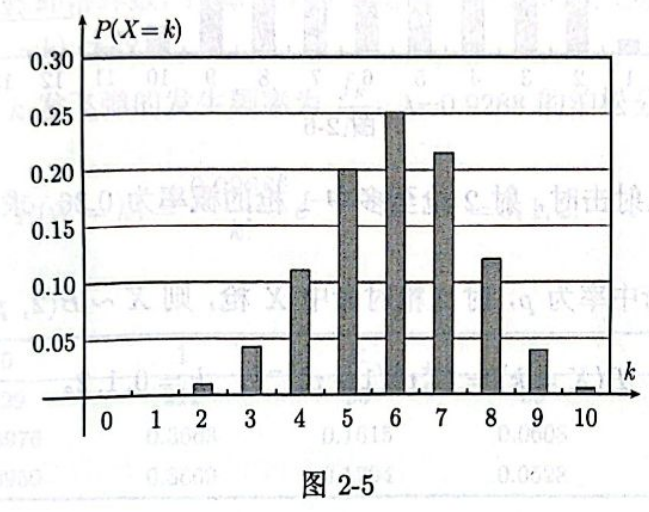
\includegraphics[scale = 0.2]{figures/figure2-5.jpg}
		\end{figure}
	\end{frame}
	
	\begin{frame}
		$p_k$最大值
		\begin{itemize}
			\item 当 $(n+1) p$ 为整数时, $p_{k}$ 在 $k=(n+1) p-1$ 和 $k=(n+1) p$ 达到最大。
			\item 当 $(n+1) p$ 不是整数时, $p_{k}$ 在 $k=[(n+1) p]$ 达到最大。其中, $[x]$ 表示不超过 $x$ 的 最大整数。
			
		\end{itemize}
	\end{frame}
	
	\begin{frame}
		例 2.6 已知某人射击时, 射 2 枪至多中 1 枪的概率为 0.36 , 求此人射 3 枪至少中 1 枪的概率。
	\end{frame}
	
	\begin{frame}
		首先观察到击中次数$X$服从二项分布$B(p, n)$。这样需要继续确定参数$p, n$。显然$n = 2,3$。这样需要继续确认$p$。
		
		\vspace*{1cm}
		解:设此人射击命中率为 $p$, 射 2 枪时命中 $X$ 枪, 则 $X \sim B(2, p)$。
		
		$$
		P(X=k)=C_{2}^{k} p^{k}(1-p)^{2-k}, \quad k=0,1,2 \text { 。 }
		$$
		
		至多中 1 枪的概率,
		
		$$
		P(X \leqslant 1)=1 - P(X > 1) =1 - P(X = 2)=1 - p ^ 2=0.36
		$$
		
		解得, $p=0.8$ 。
		
		设此人射 3 枪时命中 $Y$ 枪, 则 $Y \sim B(3,0.8)$,
		
		$$
		P(Y=k)=C_{3}^{k} 0.8^{k} 0.2^{3-k}, \quad k=0,1,2,3 \text { 。 }
		$$
		
		至少中 1 枪的概率,
		
		$$
		P(Y \geqslant 1)=1 - P(Y < 1) = 1-P(Y=0)=1-0.2^{3}=0.992 \text { 。 }
		$$
	\end{frame}
	
	\begin{frame}
		\begin{itemize}
			\item \textbf{泊松分布}
			 
			如果随机变量 $X$ 的分布律为
			
			$$
			p_{k}=P(X=k)=\frac{\lambda^{k}}{k !} e^{-\lambda}, \quad k=0,1,2, \cdots,
			$$
			
			其中 $\lambda>0$ 为常数, 则称 $X$ 服从参数为 $\lambda$ 的泊松分布, 记为 $X \sim P(\lambda)$ 。
		\end{itemize}
	\end{frame}
	
	\begin{frame}
		 例 2.7 第二次世界大战期间, 德国从本土向伦敦发射 V2飞弹, 伦敦共受 535 发飞弹袭击, 将伦敦分为 $N=576$ 个区域, 每个区域的平均落弹数 $\lambda=535 / 576=0.9288$, 以 $f_{k}$ 表示 落 $k$ 发飞弹的区域数, 有如下数据:
		 
		 \begin{tabular}{c | c c c c c c}
		 	$k$ & 0 & 1 & 2 & 3 & 4 & $\geq 5$ \\
		 	\hline 
		 	$f_k$ & 229 & 211 & 93 & 35 & 7 & 1
		 \end{tabular}
		 
		 设 $X$ 表示一个区域的落弹数, 计算一个区域落 $k$ 发飞弹的发生频率, 并与 $\lambda=0.9288$ 的 泊松分布的概率 $P(X=k)$ 比较。
	\end{frame}
	
	\begin{frame}
		解 一个区域落 $k$ 发飞弹的发生频率为 $\frac{f_{k}}{N}, \lambda=0.9288$ 的泊松分布的概率为
		
		$$
		P(X=k)=\frac{0.9288^{k}}{k !} e^{-0.9288}, \quad k=0,1,2, \cdots \text { 。 }
		$$
		
		列表计算如下:
		\begin{tabular}{c|cccccc}
			\(k\) & 0 & 1 & 2 & 3 & 4 & \(\geqslant 5\) \\
			\hline
			\(f_{k}\) & 229 & 211 & 93 & 35 & 7 & 1 \\
			\(f_{k} / N\) & 0.3976 & 0.3663 & 0.1615 & 0.0608 & 0.0122 & 0.0017 \\
			\(P(X=k)\) & 0.3950 & 0.3669 & 0.1704 & 0.0528 & 0.0122 & 0.0027 \\
		\end{tabular}
		
		可见一个区域落 $k$ 发飞弹的发生频率与泊松分布的概率整体非常吻合, 这表明一个区 域的落弹数 $X$ 非常接近泊松分布 $P(0.9288)$ 。
	\end{frame}
	
	\begin{frame}
		例 2.8 设随机变量 $X$ 服从参数为 $\lambda$ 的泊松分布, 且已知 $P(X=1)=P(X=2)$, 求 $P(X=4)$ 。
	\end{frame}
	
	\begin{frame}
		例 2.8 设随机变量 $X$ 服从参数为 $\lambda$ 的泊松分布, 且已知 $P(X=1)=P(X=2)$, 求 $P(X=4)$ 。
		
		$$
		P(X=k)=\frac{\lambda^{k}}{k !} e^{-\lambda}, \quad k=0,1,2, \cdots 。
		$$
		
		由条件 $P(X=1)=P(X=2)$, 得到
		
		$$
		\frac{\lambda^{1}}{1 !} e^{-\lambda}=\frac{\lambda^{2}}{2 !} e^{-\lambda}
		$$
		
		解得 $\lambda=2$, 因此
		
		$$
		P(X=4)=\frac{2^{4}}{4 !} e^{-2}=\frac{2}{3} e^{-2}
		$$
	\end{frame}
	
	\begin{frame}
		\begin{itemize}
			\item \textbf{几何分布}
			
			如果随机变量 $X$ 的分布律为
			
			$$
			p_{k}=P(X=k)=q^{k-1} p, \quad k=1,2, \cdots \text { 。 }
			$$
			
			其中 $0<p<1$ 为常数, $q=1-p$, 则称 $X$ 服从参数为 $p$ 的几何分布, 记为 $X \sim g(p)$ 。 验证分布律性质, 显然 $p_{k} \geqslant 0$, 且
			
			$$
			\sum_{k=1}^{\infty} p_{k}=\sum_{k=1}^{\infty} q^{k-1} p=p \sum_{k=1}^{\infty} q^{k-1}=p \frac{1}{1-q}=1 。
			$$
			
			满足分布律性质。
			
			\new{几何分布含义:}独立重复伯努利试验进行$k$次时某一事件才发生的概率。其中此特定事件在每次伯努利试验中发生概率为$p$。
		\end{itemize}
	\end{frame}
	
		
	\begin{frame}
		课外例题 2.1 独立重复扔骰子。请计算在第$k$次时第一次出现数字6的概率。
	\end{frame}
	
	\begin{frame}
		解: $X = \text{第一次出现6时扔出次数。}$$k \sim g(p = 1 / 6)$。
		
		\[
		P(X = k) = (\frac{5}{6}) ^{k - 1}\frac{1}{6}
		\]
		几何分布的\textbf{无记忆性} 
		
		在独立重复努利试验中, $A$ 首次出现时所需的试验次数服从几何分布, 若前 $t$ 次试验 $A$ 没有出现, 则再试验 $s$ 次。 $A$ 首次出现的概率与前面没有成巧 的 $t$ 次试验无关。好像把前面 $t$ 次试验给忘了, 这称为无记忆性。无记忆性的概率表达为
		
		 $$P(X=s+t \mid X>t)=P(X=s)$$
	\end{frame}
	\begin{frame}
		证明 $X \sim g(p)$, 则 $P(X=k)=q^{k-1} p$, 其中 $q=1-p, k=1,2, \cdots$ 。
		
		$$
		\begin{aligned}
			P(X>t)=\sum_{k=t+1}^{\infty} P(X=k) & =\sum_{k=t+1}^{\infty} q^{k-1} p=p \sum_{k=t+1}^{\infty} q^{k-1}=q^{t}, \\
			P(X=s+t \mid X>t) & =\frac{P(X=s+t \cap X>t)}{P(X>t)}=\frac{P(X=s+t)}{P(X>t)} \\
			& =\frac{q^{s+t-1} p}{q^{t}}=q^{s-1} p=P(X=s) .
		\end{aligned}
		$$
		
		得证。
	\end{frame}
	
	\begin{frame}
		\frametitle{连续型随机变量及其分布}
		定义 2.5 设随机变量 $X$ 的分布函数为 $F(x)$, 若存在非负可积函数 $p(x)$, 对任意实 $x$ 有
		
		$$
		F(x)=\int_{-\infty}^{x} p(t) \mathrm{d} t
		$$
		
		则称 $X$ 为连续型随机变量, 称函数 $p(x)$ 为 $X$ 的概率密度函数, 简称密度函数。
	\end{frame}
	
	\begin{frame}
		定义可见, 任何连续型随机变量的密度函数具有如下\textbf{性质}:
		\begin{enumerate}[1]
			\item $p(x) \geqslant 0$;
			\item $\int_{-\infty}^{+\infty} p(x) \mathrm{d} x=1$;  
			\item 对于任意实数 $a, b(a<b)$,
			
			$$
			P(a<X \leqslant b)=F(b)-F(a)=\int_{a}^{b} p(x) \mathrm{d} x ;
			$$
			\item 由于 $p(x)$ 为可积函数, 根据微积分性质, 分布函数 $F(x)$ 为连续函数;
			\item 若 $p(x)$ 在点 $x$ 连续, 则分布函数 $F(x)$ 在 $x$ 处可导, 且 $p(x)=F^{\prime}(x)$ 。
		\end{enumerate}
	\end{frame}
	
	\begin{frame}
		关于 (2) 的说明, $\int_{-\infty}^{+\infty} p(x) \mathrm{d} x=\lim _{x \rightarrow+\infty} \int_{-\infty}^{x} p(x) \mathrm{d} x=\lim _{x \rightarrow+\infty} F(x)=1$ 。另外, 从图形上看, (2) 表示函数 $p(x)$ 在整个 $x$ 轴上覆盖的面积为 1(图 2-7)。(3) 表 示随机变量 $X$ 在区间 $(a, b]$ 取值的概率等于密度函数 $p(x)$ 在 $(a, b)$ 覆盖的曲边梯形面积 (图 2-8)。
		\begin{figure}[htp]
			\centering
			\subfloat[2-7]{%
				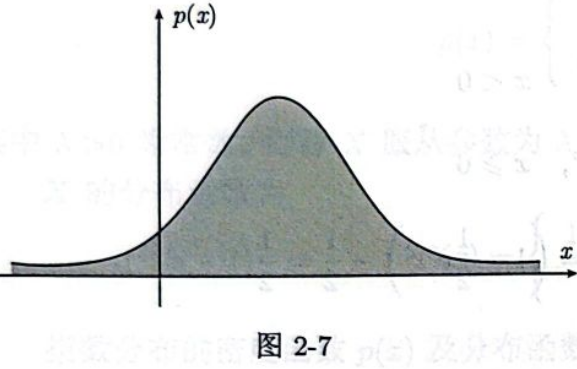
\includegraphics[width=0.4\linewidth]{figures/figure2-7}%
			}%
			\hfill%
			\subfloat[2-8]{%
				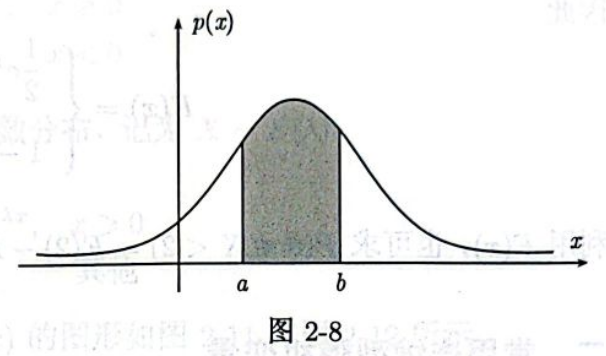
\includegraphics[width=0.4\linewidth]{figures/figure2-8}%
			}%
		\end{figure}
	\end{frame}
	
	\begin{frame}
		例 2.9 设随机变量 $X$ 的概率密度函数为
		
		$$
		p(x)=A e^{-|x|}, \quad-\infty<x<\infty,
		$$
		
		试求, (1) 常数 $A$; (2) $P(0<X<2)$; (3) 分布函数 $F(x)$ 。
	\end{frame}
	
	\begin{frame}
		分析:可由连续随机变量密度函数性质得出$A$。得到分布函数$F(x)$之后,易得$P(0 < X < 2)$,所以可以将第三问结果用于验证第二问结果。
		
		\vspace*{0.5cm}
		解 (1) $\int_{-\infty}^{+\infty} p(x) \mathrm{d} x=\int_{-\infty}^{0} A e^{x} \mathrm{~d} x+\int_{0}^{+\infty} A e^{-x} \mathrm{~d} x=2 A=1$, 因此 $A=\frac{1}{2}$ 。从而, $p(x) = \frac{1}{2} e^{-|x|},-\infty<x<\infty$ 。
		
		(2) $P(0<X<2)=\int_{0}^{2} \frac{1}{2} e^{-x} \mathrm{~d} x=\frac{1}{2}\left(1-e^{-2}\right)$ 。
		
		(3) $x<0$ 时, $F(x)=\int_{-\infty}^{x} p(x) \mathrm{d} x=\int_{-\infty}^{x} \frac{1}{2} e^{x} \mathrm{~d} x=\frac{1}{2} e^{x}$;
		
		$$
		x \geqslant 0 \text { 时, } F(x)=\int_{-\infty}^{x} p(x) \mathrm{d} x=\int_{-\infty}^{0} \frac{1}{2} e^{x} \mathrm{~d} x+\int_{0}^{x} \frac{1}{2} e^{-x} \mathrm{~d} x=1-\frac{1}{2} e^{-x},
		$$
		
		因此
		
		$$
		F(x)=\left\{\begin{array}{ll}
			\frac{1}{2} e^{x}, & x<0 \\
			1-\frac{1}{2} e^{-x}, & x \geqslant 0
		\end{array}\right. \text { 。 }
		$$
		
		利用 $F(x)$, 也可求 $P(0<X<2)=F(2)-F(0)=\left(1-\frac{1}{2} e^{-2}\right)-\frac{1}{2}=\frac{1}{2}\left(1-e^{-2}\right)$ 。
	\end{frame}
	
	\begin{frame}
	1. 均匀分布
	
	若随机变量 $X$ 的概率密度函数为
	
	$$
	p(x)=\left\{\begin{array}{cc}
		\frac{1}{b-a}, & a<x<b, \\
		0, & \text { 其他 }
	\end{array}\right.
	$$
	
	则称 $X$ 在区间 $[a, b]$ 上服从均匀分布, 记为 $X \sim U[a, b]$ 。
	
	$X$ 的分布函数为
	
	$$
	F(x)=\left\{\begin{array}{cc}
		0, & x<a \\
		\frac{x-a}{b-a}, & a \leqslant x<b . \\
		1, & x \geqslant b
	\end{array} .\right.
	$$
	
	均匀分布的密度函数 $p(x)$ 及分布函数 $F(x)$ 图形如图 2-9、图 2-10 所示。
	\begin{figure}[htp]
	\centering
	\subfloat[2-9]{%
		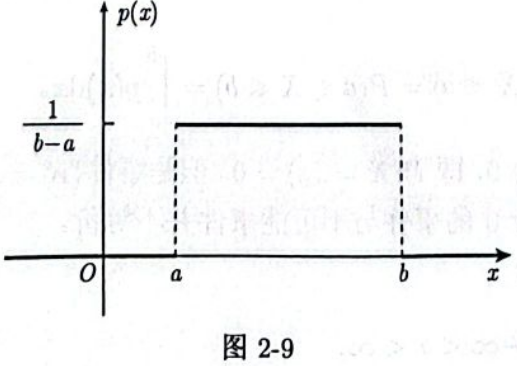
\includegraphics[width=0.35\linewidth]{figures/figure2-9}%
	}%
	\hfill%
	\subfloat[2-10]{%
		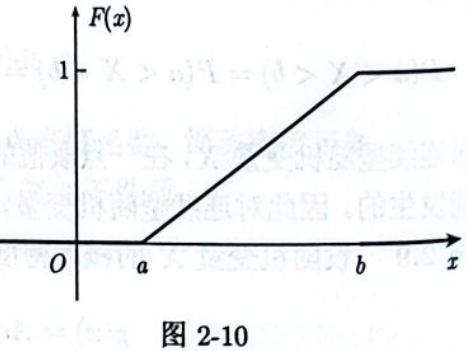
\includegraphics[width=0.35\linewidth]{figures/figure2-10}%
	}%
	\end{figure}
	\end{frame}
	
	\begin{frame}
		2. 指数分布
		
		若随机变量 $X$ 的概率密度函数为
		
		$$
		p(x)=\left\{\begin{array}{ll}
			\lambda e^{-\lambda x}, & x \geqslant 0 \\
			0, & x<0
		\end{array} .\right.
		$$
		
		其中 $\lambda>0$ 为常数, 则称 $X$ 服从参数为 $\lambda$ 的指数分布, 记为 $X \sim E(\lambda)$ 。
		
		$X$ 的分布函数为
		
		$$
		F(x)=\left\{\begin{array}{cc}
			1-e^{-\lambda x}, & x \geqslant 0 \\
			0, & \text { 其他 }
		\end{array}\right. \text {. }
		$$
		
		指数分布的密度函数 $p(x)$ 及分布函数 $F(x)$ 的图形如图 2-11 与图 2-12 所示。
	\end{frame}
	
	\begin{frame}
		\begin{figure}
			\centering
			\subfloat[2-11]{
			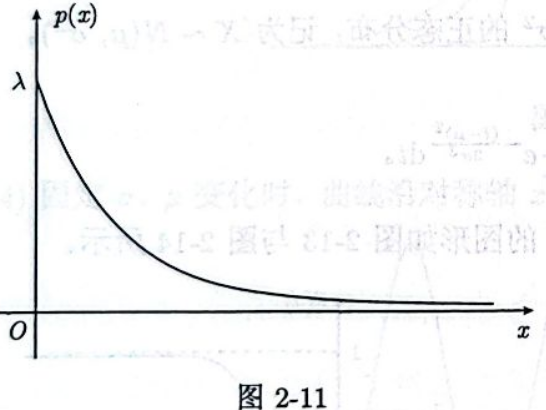
\includegraphics[width=0.5\linewidth]{figures/figure2-11}
			}
			\subfloat[2-12]{
			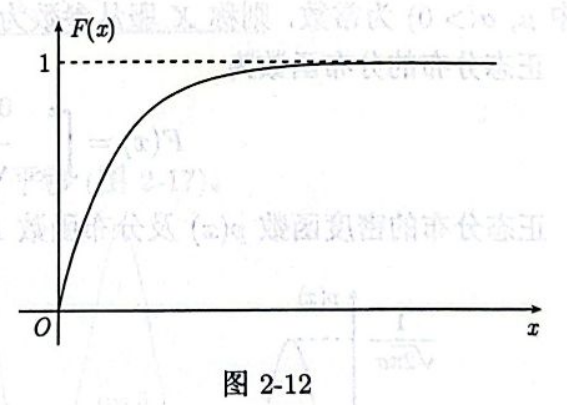
\includegraphics[width=0.5\linewidth]{figures/figure2-12}
			}
		\end{figure}
	\end{frame}
	
	\begin{frame}
		例 2.10 设某类电子元件的使用寿命 $X$ (小时) 服从参数为 $\lambda=1 / 2000$ 的指数分布, (1) 任取一只元件, 求能使用 1000 小时以上的概率; (2) 一只元件已经正常使用了 1000 小时 以上, 求还能再使用 1000 小时以上的概率。
	\end{frame}
	
	\begin{frame}
		分析:首先需计算密度函数和概率函数。第二问本质上是条件概率。
		
		解:$X$ 的分布函数为
		
		$$
		F(x)=\left\{\begin{array}{ll}
			1-e^{-\frac{1}{2000} x}, & x \geqslant 0 \\
			0, & x<0
		\end{array}\right. \text {. }
		$$
		
		(1) $P(X>1000)=1-P(X<1000)=1-F(1000)=1-\left(1-e^{-1 / 2}\right)=e^{-1 / 2}$;
		
		(2) 所求概率为
		
		$$
		\begin{aligned}
			P(X>2000 \mid X>1000) & =\frac{P(X>2000 \cap X>1000)}{P(X>1000)}=\frac{P(X>2000)}{P(X>1000)} \\
			& =\frac{1-F(2000)}{1-F(1000)}=\frac{e^{-1}}{e^{-1 / 2}}=e^{-1 / 2} 。
		\end{aligned}
		$$
		
		一只元件能使用 1000 小时以上的概率为 $e^{-1 / 2}$, 已使用了 1000 小时以上, 再使用 1000 小时以上的概率仍然为 $e^{-1 / 2}$, 这反映了指数分布的一个重要特性: 无记忆性。
	\end{frame} 
	
	\begin{frame}
		无记忆性的一般表示为
		
		$$
		P(X>s+t \mid X>s)=P(X>t)
		$$
		
		实际上,
		
		$$
		\begin{aligned}
			P(X>s+t \mid X>s) & =\frac{P(\{X>s+t\} \cap\{X>s\})}{P(X>s)}=\frac{P(X>s+t)}{P(X>s)} \\
			& =\frac{1-F(s+t)}{1-F(s)}=\frac{e^{-\lambda(s+t)}}{e^{-\lambda s}}=e^{-\lambda t}=P(X>t) 。
		\end{aligned}
		$$
	\end{frame}
	
	\begin{frame}
		3. 正态分布
		
		若随机变量 $X$ 的密度函数为
		$$
		p(x)=\frac{1}{\sqrt{2 \pi} \sigma} e^{-\frac{(x-\mu)^{2}}{2 \sigma^{2}}}, \quad-\infty<x<\infty \text { 。 }
		$$
		其中 $\mu, \sigma(>0)$ 为常数, 则称 $X$ 服从参数为 $\mu, \sigma^{2}$ 的正态分布, 记为 $X \sim N\left(\mu, \sigma^{2}\right)$ 。 正态分布的分布函数为
		$$
		F(x)=\int_{-\infty}^{x} \frac{1}{\sqrt{2 \pi} \sigma} e^{-\frac{(t-\mu)^{2}}{2 \sigma^{2}}} \mathrm{~d} t
		$$
		正态分布的密度函数 $p(x)$ 及分布函数 $F(x)$ 的图形如图 2-13,14。
	\end{frame}
	
	\begin{frame}
		\begin{figure}
			\centering
			\subfloat[2-11]{
				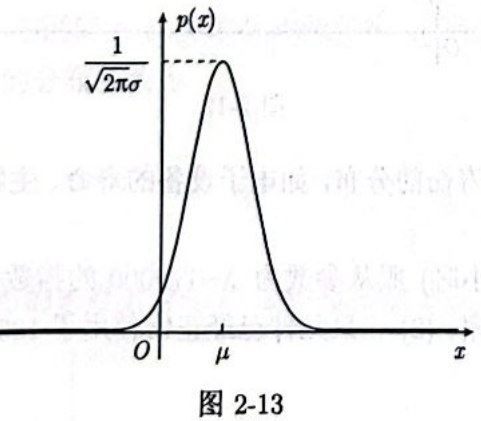
\includegraphics[width=0.5\linewidth]{figures/figure2-13}
			}
			\subfloat[2-12]{
				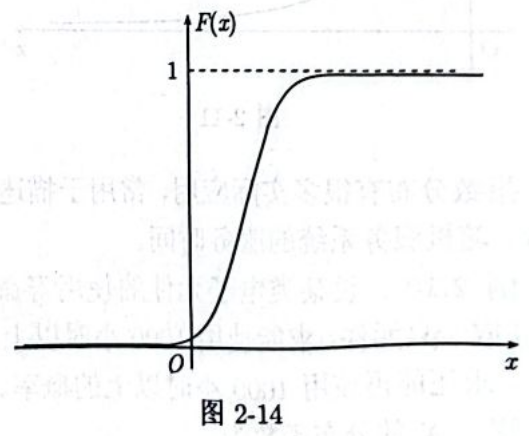
\includegraphics[width=0.5\linewidth]{figures/figure2-14}
			}
		\end{figure}
	\end{frame}
	
	\begin{frame}
		正态分布 $X \sim N\left(\mu, \sigma^{2}\right)$ 密度函数 $p(x)$ 的图形具有以下特点:
		
		(1) 曲线 $p(x)$ 关于 $x=\mu$ 对称, 且对任意 $b>0$ 有 $P(X \leqslant \mu-b)=P(X \geqslant \mu+b)$
		\begin{figure}
			\centering
			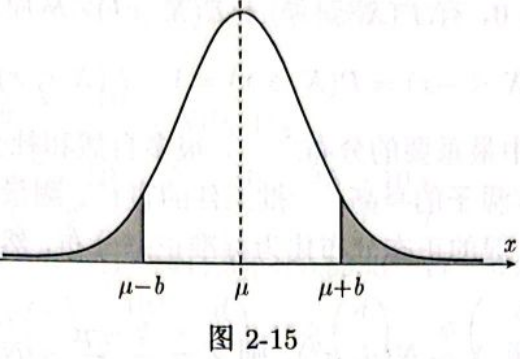
\includegraphics[scale = 0.3]{figures/figure2-15}
		\end{figure}
		(2) $x \rightarrow \pm \infty, p(x) \rightarrow 0$, 曲线以 $x$ 轴为渐近线。
	\end{frame}
	
	\begin{frame}
		(3) $x=\mu$ 时 $p(x)$ 取到最大值 $\frac{1}{\sqrt{2 \pi} \sigma}$, 由于密度图形覆盖面积总为 1 , 因此固定 $\mu$ 时, $\sigma$ 越小, 最大值越大, 图形越高越陡峭; $\sigma$ 越大, 最大值越小, 图形越低越平缓 (图 2-16)。
		\begin{figure}
			\centering
			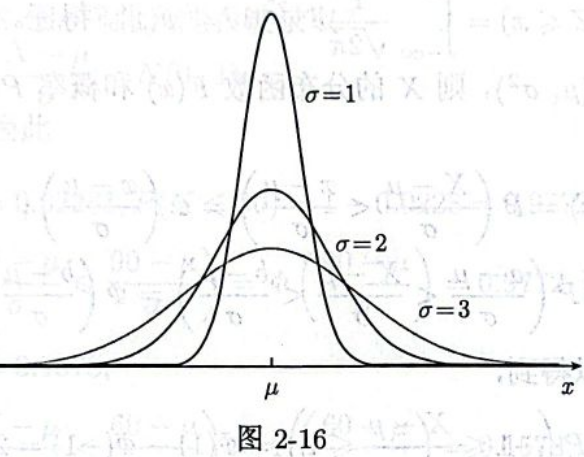
\includegraphics[scale = 0.3]{figures/figure2-16}
		\end{figure}
	\end{frame}
	
	\begin{frame}
		(4) 固定 $\sigma, \mu$ 变化时, 曲线沿对称轴 $x=\mu$ 平移 (图 2-17)。
		\begin{figure}
			\centering
			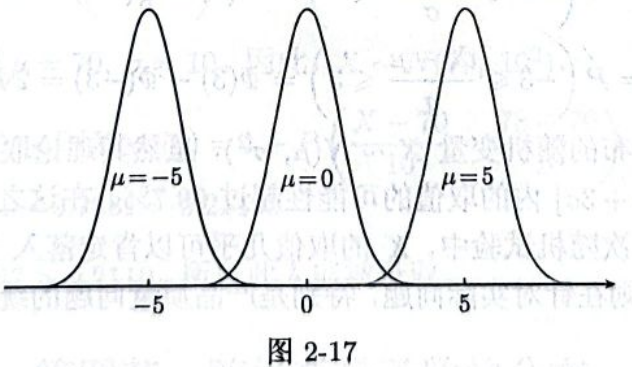
\includegraphics[scale = 0.3]{figures/figure2-17}
		\end{figure}
	\end{frame}
	
	\begin{frame}
		当 $\mu=0, \sigma=1$ 时, $X \sim N(0,1)$, 称 $X$ 服从\textbf{标准正态分布}, 其密度函数和分布函数特 别记为 $\varphi(x)$ 和 $\Phi(x)$ 。
		
		$$
		\begin{aligned}
			& \varphi(x)=\frac{1}{\sqrt{2 \pi}} e^{-\frac{x^{2}}{2}}, \\
			& \Phi(x)=\int_{-\infty}^{x} \frac{1}{\sqrt{2 \pi}} e^{-\frac{t^{2}}{2}} \mathrm{~d} t
		\end{aligned}
		$$
		
		对标准正态分布的分布函数 $\Phi(x)$, 有 $\Phi(-x)=1-\Phi(x)$ 。 事实上, 性质 (1) 中令 $\mu=0$, 有 $P(X \leqslant-b)=P(X \geqslant b)$, 从而
		
		$$
		\Phi(-x)=P(X \leqslant-x)=P(X \geqslant x)=1-P(X<x)=1-\Phi(x) 。
		$$
	\end{frame}
	
	\begin{frame}
		定理 2.1 若随机变量 $X \sim N\left(\mu, \sigma^{2}\right)$, 则 $Z=\frac{X-\mu}{\sigma} \sim N(0,1)$ 。
		
		证明 只要证明 $Z$ 的分布函数为 $\Phi(x)$ 即可。 $Z$ 的分布函数为
		
		\begin{align}
				P(Z \leqslant x)&=P\left(\frac{X-\mu}{\sigma} \leqslant x\right) \\
				&=P(X \leqslant \mu+\sigma x) \\
				&=\int_{-\infty}^{\mu+\sigma x} \frac{1}{\sqrt{2 \pi} \sigma} e^{-\frac{(t-\mu)^{2}}{2 \sigma^{2}}} \mathrm{~d} t,
		\end{align}
		
		令 $\frac{t-\mu}{\sigma}=v$, 得到, $P(Z \leqslant x)=\int_{-\infty}^{x} \frac{1}{\sqrt{2 \pi}} e^{-\frac{v^{2}}{2}} \mathrm{~d} v=\Phi(x)$, 得证。
	\end{frame}
	
	\begin{frame}
		我们可以得到,
		
		$$
		\begin{aligned}
			& P(|X-\mu| \leqslant \sigma)=P\left(-1 \leqslant \frac{X-\mu}{\sigma} \leqslant 1\right)=0.6826, \\
			& P(|X-\mu| \leqslant 2 \sigma)=P\left(-2 \leqslant \frac{X-\mu}{\sigma} \leqslant 2\right)=0.9544, \\
			& P(|X-\mu| \leqslant 3 \sigma)=P\left(-3 \leqslant \frac{X-\mu}{\sigma} \leqslant 3\right)=0.9974 。
		\end{aligned}
		$$
		正态分布随机变量在区间 $[\mu-3 \sigma, \mu+3 \sigma]$ 内的取值的可能性超过 $99.7 \%$这被称为 “ $3 \sigma$ 法则”。该法则在针对实际问题, 特别是产品质量问题的统计推断中有着重要的应 用 (图 2-18)。
	\end{frame}
	
	\begin{frame}
		\begin{figure}
			\centering
			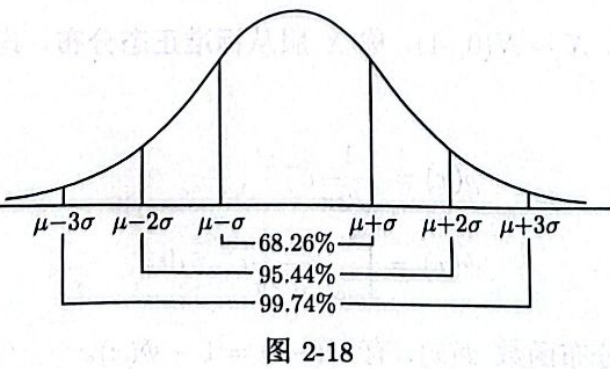
\includegraphics[scale = 0.4]{figures/figure2-18}
		\end{figure}
	\end{frame}
	
	\begin{frame}
		例 2.11 设随机变量 $X \sim N\left(10,2^{2}\right)$ 。(1) 求概率 $P(7<X<15)$; (2) 求 $d$ 的值, 使得 $P(|X-10|<d)=0.9$ 。
	\end{frame}
	
	\begin{frame}
		解 $X \sim N\left(10,2^{2}\right)$, 则 $\frac{X-10}{2} \sim N(0,1)$ 。
		
		(1) $P(7<X<15)=P\left(\frac{7-10}{2}<\frac{X-10}{2}<\frac{15-10}{2}\right)=\Phi(2.5)-\Phi(-1.5)$
		
		$$
		=\Phi(2.5)-[1-\Phi(1.5)]=0.9938-(1-0.9332)=0.927 \text { 。 }
		$$
		
		(2) $P(|X-10|<d)=P\left(\left|\frac{X-10}{2}\right|<\frac{d}{2}\right)=\Phi\left(\frac{d}{2}\right)-\Phi\left(-\frac{d}{2}\right)=2 \Phi\left(\frac{d}{2}\right)-1=0.9$, 则 $\Phi\left(\frac{d}{2}\right)=0.95$, 查表 $\Phi(1.65)=0.95, \frac{d}{2}=1.65$, 得 $d=3.3$ 。
	\end{frame}
	
	\begin{frame}[t, allowframebreaks]
		\begin{figure}[H]
			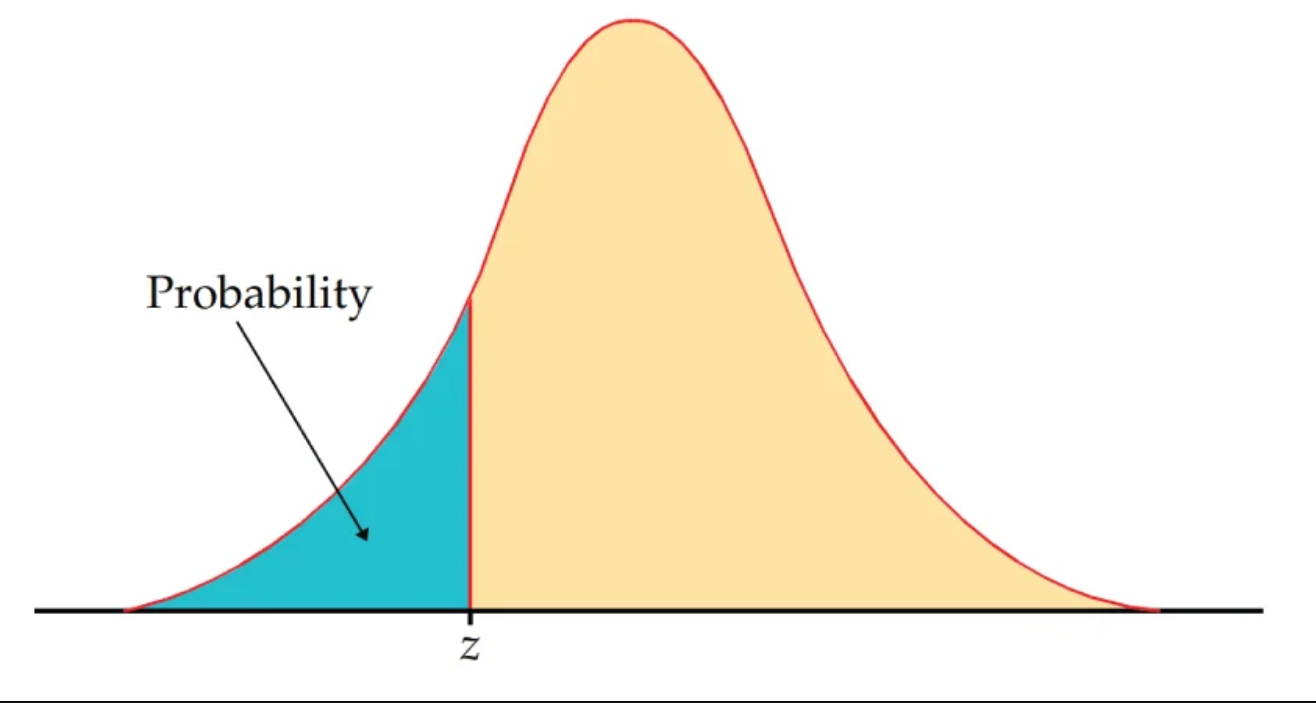
\includegraphics[scale=0.120]{figures/normal.png}
		\end{figure}
		\tiny
		\begin{longtblr}{|l|l|l|l|l|l|l|l|l|l|l|}
				\hline
				Z & 0.00 & 0.01 & 0.02 & 0.03 & 0.04 & 0.05 & 0.06 & 0.07 & 0.08 & 0.09 \\ \hline
				0.0 & 0.5000 & 0.5040 & 0.5080 & 0.5120 & 0.5160 & 0.5199 & 0.5239 & 0.5279 & 0.5319 & 0.5359 \\ \hline
				0.1 & 0.5398 & 0.5438 & 0.5478 & 0.5517 & 0.5557 & 0.5596 & 0.5636 & 0.5675 & 0.5714 & 0.5753 \\ \hline
				0.2 & 0.5793 & 0.5832 & 0.5871 & 0.5910 & 0.5948 & 0.5987 & 0.6026 & 0.6064 & 0.6103 & 0.6141 \\ \hline
				0.3 & 0.6179 & 0.6217 & 0.6255 & 0.6293 & 0.6331 & 0.6368 & 0.6406 & 0.6443 & 0.6480 & 0.6517 \\ \hline
				0.4 & 0.6554 & 0.6591 & 0.6628 & 0.6664 & 0.6700 & 0.6736 & 0.6772 & 0.6808 & 0.6844 & 0.6879 \\ \hline
				0.5 & 0.6915 & 0.6950 & 0.6985 & 0.7019 & 0.7054 & 0.7088 & 0.7123 & 0.7157 & 0.7190 & 0.7224 \\ \hline
				0.6 & 0.7257 & 0.7291 & 0.7324 & 0.7357 & 0.7389 & 0.7422 & 0.7454 & 0.7486 & 0.7517 & 0.7549 \\ \hline
				0.7 & 0.7580 & 0.7611 & 0.7642 & 0.7673 & 0.7704 & 0.7734 & 0.7764 & 0.7794 & 0.7823 & 0.7852 \\ \hline
				0.8 & 0.7881 & 0.7910 & 0.7939 & 0.7967 & 0.7995 & 0.8023 & 0.8051 & 0.8078 & 0.8106 & 0.8133 \\ \hline
				0.9 & 0.8159 & 0.8186 & 0.8212 & 0.8238 & 0.8264 & 0.8289 & 0.8315 & 0.8340 & 0.8365 & 0.8389 \\ \hline
				1.0 & 0.8413 & 0.8438 & 0.8461 & 0.8485 & 0.8508 & 0.8531 & 0.8554 & 0.8577 & 0.8599 & 0.8621 \\ \pagebreak
				1.1 & 0.8643 & 0.8665 & 0.8686 & 0.8708 & 0.8729 & 0.8749 & 0.8770 & 0.8790 & 0.8810 & 0.8830 \\ \hline
				1.2 & 0.8849 & 0.8869 & 0.8888 & 0.8907 & 0.8925 & 0.8944 & 0.8962 & 0.8980 & 0.8997 & 0.9015 \\ \hline
				1.3 & 0.9032 & 0.9049 & 0.9066 & 0.9082 & 0.9099 & 0.9115 & 0.9131 & 0.9147 & 0.9162 & 0.9177 \\ \hline
				1.4 & 0.9192 & 0.9207 & 0.9222 & 0.9236 & 0.9251 & 0.9265 & 0.9279 & 0.9292 & 0.9306 & 0.9319 \\ \hline
				1.5 & 0.9332 & 0.9345 & 0.9357 & 0.9370 & 0.9382 & 0.9394 & 0.9406 & 0.9418 & 0.9429 & 0.9441 \\ \hline
				1.6 & 0.9452 & 0.9463 & 0.9474 & 0.9484 & 0.9495 & 0.9505 & 0.9515 & 0.9525 & 0.9535 & 0.9545 \\ \hline
				1.7 & 0.9554 & 0.9564 & 0.9573 & 0.9582 & 0.9591 & 0.9599 & 0.9608 & 0.9616 & 0.9625 & 0.9633 \\ \hline
				1.8 & 0.9641 & 0.9649 & 0.9656 & 0.9664 & 0.9671 & 0.9678 & 0.9686 & 0.9693 & 0.9699 & 0.9706 \\ \hline
				1.9 & 0.9713 & 0.9719 & 0.9726 & 0.9732 & 0.9738 & 0.9744 & 0.9750 & 0.9756 & 0.9761 & 0.9767 \\ \hline
				2.0 & 0.9772 & 0.9778 & 0.9783 & 0.9788 & 0.9793 & 0.9798 & 0.9803 & 0.9808 & 0.9812 & 0.9817 \\ \hline
				2.1 & 0.9821 & 0.9826 & 0.9830 & 0.9834 & 0.9838 & 0.9842 & 0.9846 & 0.9850 & 0.9854 & 0.9857 \\ \hline
				2.2 & 0.9861 & 0.9864 & 0.9868 & 0.9871 & 0.9875 & 0.9878 & 0.9881 & 0.9884 & 0.9887 & 0.9890 \\ \hline
				2.3 & 0.9893 & 0.9896 & 0.9898 & 0.9901 & 0.9904 & 0.9906 & 0.9909 & 0.9911 & 0.9913 & 0.9916 \\ \hline
				2.4 & 0.9918 & 0.9920 & 0.9922 & 0.9925 & 0.9927 & 0.9929 & 0.9931 & 0.9932 & 0.9934 & 0.9936 \\ \hline
				2.5 & 0.9938 & 0.9940 & 0.9941 & 0.9943 & 0.9945 & 0.9946 & 0.9948 & 0.9949 & 0.9951 & 0.9952 \\ \hline
				2.6 & 0.9953 & 0.9955 & 0.9956 & 0.9957 & 0.9959 & 0.9960 & 0.9961 & 0.9962 & 0.9963 & 0.9964 \\ \hline
				2.7 & 0.9965 & 0.9966 & 0.9967 & 0.9968 & 0.9969 & 0.9970 & 0.9971 & 0.9972 & 0.9973 & 0.9974 \\ \hline
				2.8 & 0.9974 & 0.9975 & 0.9976 & 0.9977 & 0.9977 & 0.9978 & 0.9979 & 0.9979 & 0.9980 & 0.9981 \\ \hline
				2.9 & 0.9981 & 0.9982 & 0.9982 & 0.9983 & 0.9984 & 0.9984 & 0.9985 & 0.9985 & 0.9986 & 0.9986 \\ \hline
				3.0 & 0.9987 & 0.9987 & 0.9987 & 0.9988 & 0.9988 & 0.9989 & 0.9989 & 0.9989 & 0.9990 & 0.9990 \\ \hline
		\end{longtblr}
	\end{frame}
	
	\begin{frame}
		例 2.12 某单位计划招聘 155 名员工, 按考试成绩从高分到低分依次录取。现有 526 人报名, 假设报名者的成绩 $X \sim N\left(\mu, \sigma^{2}\right)$ 。已知报名者中 90 分以上有 12 人, 60 分以下有 83 人。已知某人成绩为 78 分, 问此人能否被录取?
	\end{frame}
	
	\begin{frame}
		解 $X \sim N\left(\mu, \sigma^{2}\right), \frac{X-\mu}{\sigma} \sim N(0,1)$ 。
		
		90 分以上有 12 人, 因此
		
		$$
		\begin{aligned}
			& P(X>90)=\frac{12}{526}=0.02281, P(X \leqslant 90)=1-0.0228=0.9772, \\
			& P(X \leqslant 90)=P\left(\frac{X-\mu}{\sigma} \leqslant \frac{90-\mu}{\sigma}\right)=\Phi\left(\frac{90-\mu}{\sigma}\right)=0.9772, \text { 查表, } \\
			&\frac{90-\mu}{\sigma}=2, \\
			& P(X<60)=\frac{83}{526}=0.1578, \\
			& P(X<60)=P\left(\frac{X-\mu}{\sigma}<\frac{60-\mu}{\sigma}\right)=\Phi\left(\frac{60-\mu}{\sigma}\right)=0.1578, \\
			& \Phi\left(-\frac{60-\mu}{\sigma}\right)=1-\Phi\left(\frac{60-\mu}{\sigma}\right)=1-0.1578=0.8422, \text { 查表, }\\
			&\frac{60-\mu}{\sigma}=1,
		\end{aligned}
		$$
		
		
	\end{frame}
	
	\begin{frame}
		解 $\mu, \sigma$ 的方程组, 得到 $\mu=70, \sigma=10$ 。因此, $X \sim N\left(70,10^{2}\right)$,
		
		$$
		\begin{aligned}
			P(X \geqslant 78) & =1-P(X<78)=1-P\left(\frac{X-70}{10}<\frac{78-70}{10}\right)=1-\Phi(0.8) \\
			& =1-0.7881=0.2119 \text { 。 }
		\end{aligned}
		$$
		
		而录取率为 $\frac{155}{526}=0.2947>0.2119$, 所以此人能被录取。
	\end{frame}
	
	\begin{frame}
		\frametitle{随机变量函数的分布}
		一、离散型随机变量的函数
		
		设 $X$ 是离散型随机变量, 其分布律为
		\begin{center}
			\begin{tabular}{l|lllll}
				$X$ & $x_{1}$ & $x_{2}$ & $\ldots$ & $x_{n}$ & $\ldots$ \\
				\hline
				$P$ & $p_{1}$ & $p_{2}$ & $\ldots$ & $p_{n}$ & $\ldots$ \\
			\end{tabular}
		\end{center}
		对于 $X$ 的函数 $Y=g(X), Y$ 也是离散型随机变量, 求 $Y$ 的分布律。
		
		当 $X$ 取值 $x_{k}$ 时, $Y=g(X)$ 取值 $y_{k}=g\left(x_{k}\right), k=1,2, \cdots$ 。
		
		(1) 若 $y_{1}, y_{2}, \cdots, y_{n}, \cdots$ 的取值互不相同, 则 $X=x_{k}$ 时, 一定有 $Y=y_{k}=g\left(x_{k}\right)$, 所以 $Y=y_{k}$ 的概率与 $X=x_{k}$ 的概率相同, 即
		
		$$
		P\left(Y=y_{k}\right)=P\left(Y=g\left(x_{k}\right)\right)=P\left(X=x_{k}\right)=p_{k},
		$$
		
		从而得到 $Y$ 的分布律:
	\end{frame}
	
	\begin{frame}
		\begin{center}
			\begin{tabular}{l|lllll}
				$Y$ & $y_{1}$ & $y_{2}$ & $\cdots$ & $y_{n}$ & $\cdots$ \\
				\hline
				$P$ & $p_{1}$ & $p_{2}$ & $\cdots$ & $p_{n}$ & $\cdots$ \\
			\end{tabular}
		\end{center}
		(2) 若 $y_{1}, y_{2}, \cdots, y_{n}, \cdots$ 的取值有相同的, 则应把相同的 $y_{k}$ 对应的概率相加, 作为 $P\left(Y=y_{k}\right)$ 的概率取值。即
		
		$$
		P\left(Y=y_{k}\right)=\sum_{i: y_{k}=g\left(x_{i}\right)} P\left(X=x_{i}\right),
		$$
		
		同样得到 $Y$ 的分布律。
	\end{frame}

	\begin{frame}
			例 2.13 设随机变量 $X$ 的分布律为
		\begin{center}
			\begin{tabular}{c|ccccc}
				$X$ & -1 & 0 & 1 & 2 & 3 \\
				\hline
				$P$ & 0.2 & 0.2 & 0.1 & 0.3 & 0.2 \\
			\end{tabular}
		\end{center}
		求 $Y=(X-1)^{2}$ 的分布律。
	\end{frame}
	
	\begin{frame}
		解 $X$ 取值 $-1,0,1,2,3$ 时, $Y$ 依次取值 4, 1, 0, 1, 4, 于是,
		
		$$
		\begin{aligned}
			& P(Y=0)=P(X=1)=0.1 \\
			& P(Y=1)=P(X=0)+P(X=2)=0.2+0.3=0.5 \\
			& P(Y=4)=P(X=-1)+P(X=3)=0.2+0.2=0.4 。
		\end{aligned}
		$$
		
		所以, 得到 $Y$ 的分布律如下:
		\begin{center}
			\begin{tabular}{c|ccc}
				$Y$ & 0 & 1 & 4 \\
				\hline
				$P$ & 0.1 & 0.5 & 0.4 \\
			\end{tabular}
		\end{center}
	\end{frame}
	
	\begin{frame}
		例 2.14 设随机变量 $X$ 的分布律为 $P(X=k)=1 / 2^{k}, k=1,2, \cdots$, 求 $Y=\sin \left(\frac{\pi}{2} X\right)$ 的概率分布。
	\end{frame}
	
	\begin{frame}
		解 $X$ 与 $Y$ 的取值关系如下表, $Y$ 的取值具有周期性, $Y$ 只取 $-1,0,1$ 三个值,
		\begin{center}
			\begin{tabular}{c|cccccccccc}
				$X$ & 1 & 2 & 3 & 4 & 5 & 6 & 7 & 8 & 9 & $\cdots$ \\
				\hline
				$P$ & 1 & 0 & -1 & 0 & 1 & 0 & -1 & 0 & 1 & $\cdots$ \\
			\end{tabular}
		\end{center}
		$$
		\begin{aligned}
			P(Y=-1) & =P(X=3)+P(X=7)+P(X=11)+\cdots \\
			& =\frac{1}{2^{3}}+\frac{1}{2^{7}}+\frac{1}{2^{11}}+\cdots=\frac{1 / 2^{3}}{1-1 / 2^{4}}=\frac{2}{15}, \\
			P(Y=0) & =P(X=2)+P(X=4)+P(X=6)+\cdots \\
			& =\frac{1}{2^{2}}+\frac{1}{2^{4}}+\frac{1}{2^{6}}+\cdots=\frac{1 / 2^{2}}{1-1 / 2^{2}}=\frac{1}{3}, \\
			P(Y=1) & =P(X=1)+P(X=5)+P(X=9)+\cdots \\
			& =\frac{1}{2}+\frac{1}{2^{5}}+\frac{1}{2^{9}}+\cdots=\frac{1 / 2}{1-1 / 2^{4}}=\frac{8}{15} 。
		\end{aligned}
		$$
		
		得到 $Y$ 的分布律
		\begin{center}
			\begin{tabular}{c|ccc}
				$Y$ & -1 & 0 & 1 \\
				\hline
				$P$ & $2 / 15$ & $1 / 3$ & $8 / 15$ \\
			\end{tabular}
		\end{center}
	\end{frame}
	
	\begin{frame}
		二、连续型随机变量的函数
		
		设 $X$ 是连续型随机变量, $y=g(x)$ 为连续实函数, 则 $Y=g(X)$ 也是连续型随机变量。 已知 $X$ 的密度函数 $p_{X}(x)$, 求 $Y$ 的密度函数 $p_{Y}(y)$ 。
		
		常用的方法是分布函数法, 即先求 $Y$ 的分布函数 $F_{Y}(y)$,
		
		$$
		F_{Y}(y)=P(Y \leqslant y)=P(g(X) \leqslant y)=\int_{x: g(x) \leqslant y} p_{X}(x) \mathrm{d} x,
		$$
		
		然后, $p_{Y}(y)=F_{Y}^{\prime}(y)$ 。
	\end{frame}
	
	\begin{frame}
		例 2.15 设随机变量 $X$ 服从 $[-1,1]$ 上的均匀分布, $Y=2 X+1$, 求 $Y$ 的密度函数 $p_{Y}(y)$ 。
	\end{frame}
	
	\begin{frame}
		解 $X$ 的密度函数 $p_{X}(x)=\left\{\begin{array}{cc}1 / 2, & -1 \leqslant x \leqslant 1 \\ 0, & \text { 其他 }\end{array}\right.$, 记 $Y$ 的分布函数为 $F_{Y}(y)$, 由于 $Y$ 的可能取值范围是 $[-1,3]$, 因此
		
		$y<-1$ 时,
		
		$$
		F_{Y}(y)=P(Y \leqslant y)=0
		$$
		
		$-1 \leqslant y \leqslant 3$ 时,
		
		$$
		\begin{aligned}
			F_{Y}(y) & =P(Y \leqslant y)=P(2 X+1 \leqslant y) \\
			& =P\left(X \leqslant \frac{1}{2} y-\frac{1}{2}\right)=\int_{-1}^{\frac{1}{2} y-\frac{1}{2}} \frac{1}{2} \mathrm{~d} x=\frac{1}{4}(y+1),
		\end{aligned}
		$$
		
		$y>3$ 时,
		
		$$
		F_{Y}(y)=P(Y \leqslant y)=1 \text { 。 }
		$$
		
		得到
		$$
		p_{Y}(y)=F_{Y}^{\prime}(y)=\left\{\begin{array}{cc}
			\frac{1}{4}, & -1 \leqslant y \leqslant 3 \\
			0, & \text { 其他 }
		\end{array},\right.
		$$
		
		$Y$ 仍然服从均匀分布, $Y \sim U[-1,3]$ 。
	\end{frame}
	
	\begin{frame}
		例 2.16 设随机变量 $X$ 的概率密度为 $p_{X}(x),-\infty<x<\infty$, 求 $Y=X^{2}$ 的密度函数 $p_{Y}(y)$ 。
	\end{frame}
	
	\begin{frame}
		解:先求 $Y$ 的分布函数 $F_{Y}(y) \circ Y$ 的可能取值范围 $[0,+\infty)$, 因此 $y<0$ 时,
		
		$$
		F_{Y}(y)=P(Y \leqslant y)=0,
		$$
		
		$y>0$ 时,
		
		$$
		\begin{aligned}
			F_{Y}(y) & =P(Y \leqslant y)=P\left(X^{2} \leqslant y\right) \\
			& =P(-\sqrt{y} \leqslant X \leqslant \sqrt{y})=F_{X}(\sqrt{y})-F_{X}(-\sqrt{y}) 。
		\end{aligned}
		$$
		
		对 $F_{Y}(y)$ 求导,
		
		$$
		p_{Y}(y)=F_{Y}^{\prime}(y)=\left\{\begin{array}{cc}
			\frac{1}{2 \sqrt{y}}\left[p_{X}(\sqrt{y})+p_{X}(-\sqrt{y})\right], & y>0 \\
			0, & y \leqslant 0
		\end{array} .\right.
		$$
		
		若已知 $X$ 的概率密度代入上式, 便可求 $Y=X^{2}$ 的概率密度。例如, $X$ 服从标准正态 分布, $X$ 的概率密度 $\varphi(x)=\frac{1}{\sqrt{2 \pi}} e^{-\frac{x^{2}}{2}}$, 代入可得
		
	\end{frame}
	
	\begin{frame}
			$$
		p_{Y}(y)=\left\{\begin{array}{cc}
			\frac{1}{\sqrt{2 \pi y}} e^{-\frac{y}{2}}, & y>0 \\
			0, & y \leqslant 0
		\end{array}\right. \text { 。 }
		$$
		
		称 $Y$ 服从自由度为 1 的 $\chi^{2}$ 分布, $\chi^{2}$ 分布是统计学中的一个重要分布。
	\end{frame}
	
	\begin{frame}
		定理 2.2 设随机变量 $X$ 的可能取值范围为 $(a, b), X$ 的概率密度为 $p_{X}(x), a<x<$ $b$ (其中 $a$ 可为 $-\infty, b$ 可为 $+\infty$ ), 设函数 $y=g(x)$ 处处可导, 且恒有 $g^{\prime}(x)>0$ [或恒有 $\left.g^{\prime}(x)<0\right]$, 则 $Y=g(X)$ 为连续型随机变量, 其概率密度为
		
		$$
		p_{Y}(y)=\left\{\begin{array}{cl}
			p_{X}\left[g^{-1}(y)\right] \cdot\left|\left[g^{-1}(y)\right]^{\prime}\right|, & \alpha<y<\beta \\
			0, & \text { 其他 }
		\end{array}\right. \text { 。 }
		$$
		
		其中, $\alpha=\min \{g(a), g(b)\}, \beta=\max \{g(a), g(b)\}, g^{-1}(y)$ 为 $y=g(x)$ 的反函数。
	\end{frame}
	
	\begin{frame}
		例 2.17 设随机变量 $X \sim N\left(\mu, \sigma^{2}\right)$, 求 $X$ 的线性函数 $Y=a X+b(a \neq 0)$ 的密度函 数 $p_{Y}(y)$ 。
	\end{frame}
	
	\begin{frame}
		解:$X$ 的密度函数为
		
		$$
		P_{X}(x)=\frac{1}{\sqrt{2 \pi} \sigma} e^{-\frac{(x-\mu)^{2}}{2 \sigma^{2}}}, \quad-\infty<x<+\infty,
		$$
		
		由 $y=a x+b$ 严格单调, 解得反函数
		
		$$
		x=g^{-1}(y)=\frac{y-b}{a}, \quad\left[g^{-1}(y)\right]^{\prime}=\frac{1}{a},
		$$
		
		根据定理 $2.2, Y=a X+b$ 的密度为
		
		$$
		\begin{aligned}
			p_{Y}(y) & =p_{X}\left(g^{-1}(y)\right) \cdot\left|\left[g^{-1}(y)\right]^{\prime}\right|=p_{X}\left(\frac{y-b}{a}\right) \cdot\left|\frac{1}{a}\right|, \\
			& =\frac{1}{\sqrt{2 \pi} \sigma} e^{-\frac{\left(\frac{y-b}{a}-\mu\right)^{2}}{2 \sigma^{2}}} \cdot\left|\frac{1}{a}\right|=\frac{1}{\sqrt{2 \pi}|a| \sigma} e^{-\frac{|y-(a \mu+b)|^{2}}{2 a^{2} \sigma^{2}}} .
		\end{aligned}
		$$
		
		可见, $Y$ 仍然服从正态分布, $Y \sim N\left(a \mu+b, a^{2} \sigma^{2}\right)$ 。
		
		上述结论中, 对 $X \sim N\left(\mu, \sigma^{2}\right)$, 令 $a=\frac{1}{\sigma}, b=-\frac{\mu}{\sigma}$, 则有 $a \mu+b=0, a^{2} \sigma^{2}=1, Y=$ $a X+b=\frac{X-\mu}{\sigma} \sim N(0,1)$.(定理 2.1)
	\end{frame}
\end{document}